\documentclass[letter,10pt]{article}
\usepackage[utf8]{inputenc}
\usepackage{graphicx}
\usepackage{natbib}
\usepackage{hyperref}
\usepackage{courier}
\usepackage[margin=0.75in]{geometry}
\usepackage[table,svgnames]{xcolor}
\usepackage{multirow}
\usepackage{tabu}
\usepackage{float} \usepackage{listings}
\usepackage{xspace} 
\bibliographystyle{unsrtnat}
\definecolor{HeaderColor}{rgb}{0.8, 0.8, 0.95}
\setlength{\parindent}{0pt}
\setlength{\parskip}{6pt}

\usepackage[T1]{fontenc}
\usepackage[utf8]{inputenc}
\usepackage{authblk}

\author[1,2]{Dimitri Yatsenko\thanks{dvyatsen@bcm.edu}}
\author[1,2]{Edgar Y. Walker}
\author[1,2]{Andreas S. Tolias}
\affil[1]{Department of Neuroscience, Baylor College of Medicine, Houston, Texas, USA}
\affil[2]{Vathes LLC, Houston, Texas, USA}

\renewcommand\Authands{ and }
\newcommand{\datajoint}{DataJoint\xspace}
\date{\today\\Revision 0.1}


\graphicspath{{./figures/}}

\lstset{
    backgroundcolor=\color{AliceBlue},
    tabsize=4,
    basicstyle=\ttfamily\small,
    breaklines=true
    aboveskip={0.5\baselineskip},
    columns=fixed,
    frame=none,
    captionpos=b,
    showstringspaces=false,
    extendedchars=false,
    breaklines=true,
    numbers=none,
    showtabs=false,
    showspaces=false,
    showstringspaces=false,
    framextopmargin=50pt,
    xleftmargin=2pt,
    framexleftmargin=2pt,
    identifierstyle=\color{Black},
    keywordstyle=\bfseries\color{DarkSlateBlue},
    commentstyle=\color{Sienna}\itshape\small,
    stringstyle=\color{Indigo},
    numberstyle=\tiny\color{DarkGray}}

\lstdefinelanguage{dj}{
  keywords={int, smallint, char, varchar, enum, unsigned, date, year, decimal},
  keywordstyle=\color{blue},
  keywords=[2]{boolean, string, number, objectid},
  keywordstyle=[2]\color{green}\bfseries,
  identifierstyle=\color{Black},
  sensitive=true,
  morecomment=[l][\color{Teal}\bfseries]{::},
  morecomment=[l][\color{Sienna}\itshape\small]{\#},
  stringstyle=\color{Indigo},
  morestring=[b]',
  morestring=[b]"
}

\newfloat{lstfloat}{htbp}{lop}
%\floatname{lstfloat}{Listing}

\title{\datajoint: A Simpler Relational Data Model}

\begin{document}

\maketitle
\begin{abstract}
We propose a simplified and conceptually refined relational data model complete with a language for schema definition and data queries as well as  diagramming notation for visualizing relationships among the data.  
Named \datajoint, the model adheres to the principle of \emph{entity normalization}, which requires that all data --- both stored and derived --- exist in the form of sets of entities belonging to well-defined entity types.  
\datajoint's data query language is an algebra of five operators that provide equal capabilities to those of other relational query languages with greater clarity due to entity normalization. 
Practical implementations of \datajoint have been tested and adopted for scientific data pipelines by a number of leading science labs, allowing interaction with scientific data that is more fluent than with other data management solutions.
\end{abstract}
\tableofcontents 

\twocolumn

\section{Core Concepts}
\subsection{The Relational Data Model}
The relational data model \citep{codd_relational_1970} provides the most rigorous approach to structuring stored data as well as the most precise approach to querying data.  
The relational data model is defined by the principles of data representation, domain constraints, uniqueness constraints, referential constraints, and declarative queries summarised in Table \ref{tab:core}.

\tabulinesep=6pt
\begin{table*}[ht]
\begin{tabu}{|X|}
\hline
{\bf Data representation.} Data are represented and manipulated in the form of \emph{relations}. 
A relation is a \emph{set} (\emph{i.e.}\ an unordered collection) of \emph{tuples} of values for each of the respective named \emph{attributes} of the relation.
\emph{Base relations} represent stored data while \emph{derived relations} are formed from base relations as a result of data queries.
A collection of base relations with their attributes, domain constraints, uniqueness constraints, and referential constraints is called a \emph{schema}.

\\
{\bf Domain constraints.} Attribute values are drawn from corresponding attribute \emph{domains}, \emph{i.e.}\ predefined sets of values.
Attribute domains may not include other relations, ensuring that the relational model is essentially flat with no nesting data structures.

\\
{\bf Uniqueness constraints.} Tuples within relations are addressed by values of their attributes.
To identify and relate data elements, \emph{uniqueness constraints} on a subset of attributes may be imposed so that no two tuples can have the same values of these attributes.  The set of attributes with a uniqueness constraints are referred to as a \emph{key}. One in a relation key may be designated as the \emph{primary key} for the relation to serve for referencing elements in a relation.

\\
{\bf Referential constraints.} Associations among data are established by means of \emph{referential constraints} in the form of \emph{foreign keys}. 
Referential constraints prohibit tuples in one relation unless the referenced relation already contains tuples with matching values of corresponding attributes. 

\\
{\bf Declarative queries.} \emph{Queries} produce derived relations from base relations and retrieve the result.  
\emph{Query expressions} provide declarative specifications for retrieved data rather than procedural specifications typical of other data models. 
Formal languages for query expressions include \emph{relational algebra} and \emph{relational calculus}.  
\\
\hline
\end{tabu}
\caption{Core principles of the relational data model.}
\label{tab:core}
\end{table*}

Popular implementations of the relational data model rely on the Structured Query Language (SQL).
SQL comprises distinct sublanguages for schema definition, data manipulation, and data queries.
SQL so thoroughly dominates in the space of relational databases that, in casual discourse, SQL and the relational data model have become conflated. 

\datajoint is a clean, consistent, and conceptually refined implementation of the relational data model adhering faithfully to its core principles.
Its introduction is motivated by the need for expressive and rigorous  constructs for database programming in scientific computing.

\datajoint comprises 
\begin{itemize}
\item a \emph{schema definition language} (Sections \ref{sec:def1} and \ref{sec:def2})
\item a \emph{data manipulation language} (Section \ref{sec:manip})
\item a \emph{data query language} (Section \ref{sec:query})
\item diagramming notation for visualizing relationships between modeled entities (Section \ref{sec:diag}).
\end{itemize}

Relations are often visualized as \emph{tables} with attributes corresponding to \emph{columns} and tuples corresponding to \emph{rows}.  
In particular, SQL uses these terms rather than those of the formal relational model.  
Table \ref{tab:terms} correlates equivalent terms used in different variants of the relational data model.

\tabulinesep=6pt
\begin{table*}[ht]
   \rowcolors{1}{white}{gray!20}
   \begin{tabu}{|X[1,c,p]| X[1,c]| X[1,c]| X[1,c]|}
   \hline
   \rowcolor{HeaderColor}
   {\bf Relational} & {\bf ERM} & {\bf SQL} & {\bf \datajoint}  \\
   \cellcolor{white} & entity set & \cellcolor{white} & \cellcolor{white} \\
   \multirow{-2}{*}{relation}  & relationship set  & \multirow{-2}{*}{table}  &  \multirow{-2}{*}{entity set} \\
   tuple       & entity           & row    & entity \\
   domain      & value set        & data type & data type \\
   attribute   & attribute        & column {\em or} field    & attribute \\
   attribute value & attribute value  & field value & attribute value \\
   primary key & primary key & primary key & primary key \\
   foreign key & foreign key & foreign key & foreign key {\em or} dependency \\
   schema      & schema      &  schema  &  schema \\
   relational expression \par {\em or} derived relation &  data query & {\tt SELECT} statement & query expression \\
   \hline
   \end{tabu}
\caption{Corresponding terms used in variants of relational models.}
\label{tab:terms}
\end{table*}

\subsection{Conceptual Ambiguity}
The relational model is abstract and semantically unconstrained, providing few guidelines for translating problems into database schemas or for forming valid queries. 
Learning to design and query databases for practical problems requires \emph{conceptual clarification}: developing intuition and techniques for mapping real-world rules onto the concepts of the relational data model from Table \ref{tab:core}.

A set of formal rules known as \emph{normal forms} have been devised to test whether a particular schema meets basic quality requirements that preclude redundancies in data storage and avoid anomalies in data manipulations \citep{kent-1983-simple}.  
Relying on the mathematical concept of {\em functional dependencies} among the attributes, normal forms remain abstract and provide no conceptual clarification. 
When a schema does not meet the normal forms, it is considered \emph{unnormalized}; whereas redesigning schemas to meet these tests is called \emph{normalization}.
SQL does not provide mechanisms for enforcing or diagnosing normalization in its data definition language. 
It takes considerable training to educate database programmers about the design of normalized schemas in the general case. 

For data queries, the relational data model provides few constraints as to what constitutes a valid or meaningful query, allowing unlimited freedom to compare, match, and combine attributes of relations regardless of their semantic compatibility.

New practitioners enter the field of database programming with their diverse backgrounds and mindsets, conceiving of database tables as spreadsheets with arbitrary semantics of rows and columns.  
Only with experience in more sophisticated designs, do they develop, mostly implicitly, various semantic mappings of real-world information motifs and database design pattens.

The overall lack of semantic constraints in the relational data model and SQL in particular leaves great freedom to experienced developers with honed conceptual skills. But it also allows for a great diversity of incompatible approaches to schema design and data queries and lengthens the path from mediocrity to proficiency.

\subsection{Entity-Relationship Model}
The most successful effort to clarify the relational data model began with the Entity-Relationship Model (ERM) \citep{chen_entity_1976}.  
The ERM provides 
\begin{enumerate}
\item a method for problem analysis for schema design 
\item diagramming notation for schema design 
\item constraints for meaningful queries
\end{enumerate}

The central concept in ERM is that of an {\em entity set}: an unordered collection of identifiable items (entities) in the modeled world that share the same set of attributes, are distinguished from each other by the same \emph{primary key}, and can participate in the same types of relationships with other entity sets. 
In ERM, all base relations are either entity sets or \emph{relationship sets} between entity sets; these terms effectively subsume the term \emph{relation} (Table \ref{tab:terms}).

ERM diagramming notation depicts entity sets and relationship sets, turning ERM into an effective tool for \emph{conceptual modeling} and communication between database designers, customers, and managers.
For example, Figure \ref{fig:erm-notation} depicts a simple entity-relationship diagram for a university student database with two entity sets, {\tt Student} and {\tt Department} and the relationship {\tt majors in} between them.

\begin{figure}
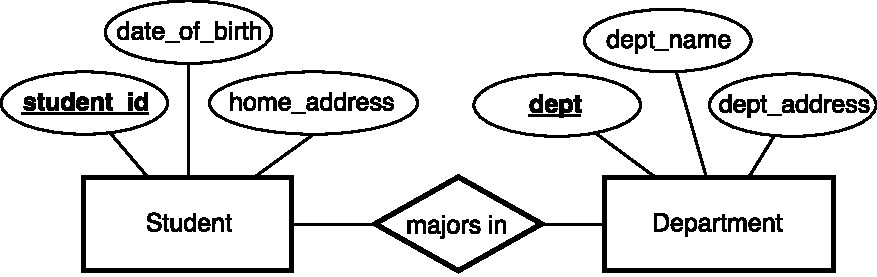
\includegraphics[width=\columnwidth]{student-dept-erd.pdf}
\caption{The entity-relationship diagram of a database schema model university departments, students,  and their major department using ERM diagramming notation.}
\label{fig:erm-notation}
\end{figure}


A \emph{relationship set} is a collection of associations linking entities from two or more entity sets and sharing the same set of attributes. 
These associations take the form of referential constraints (foreign keys) between relationships sets and entity sets.
Although the ERM is mostly known for its approach to schema design, it also prescribes methods to form valid data queries: Queries must rely on foreign keys to match entities through the relationships in which they participate. 

ERM was proposed as a complete data model in its own right but its conceptual refinements were never translated into a practical programming language and, today, ERM is best known as a diagramming technique only.  
Formal courses in database programming prescribe a two-phased approach to database design: \emph{conceptual modeling} using a diagramming tool such as ERM followed by translation or (\emph{logical  design}) into a relational database schema and SQL \citep{elmasri-2015-fundamentals, coronel-2016-database}. 
Trained database designers mentally internalize ERM principles in their approach to schema design and queries.
They often explicitly or mentally categorize tables as either ``entity tables'' or ``relationship tables'' even though SQL makes no such distinction. 
Such partitioning of entities and their relationships onto distinct relations in a database schema yields designs that are naturally normalized, \emph{i.e.}\ they pass the criteria of normal forms. 
ERM-based designs tend to naturally produce database schemas that already  meet rules of database normalization from formal relational database theory so that practicing database developers rarely need to recall the definitions of normal forms from their formal academic training.
When using the ERM approach, the problem of database normalization is translated into a more relatable problem of correctly distinguishing entities in the modeled world.  
We will refer to this approach to database normalization as \emph{entity normalization} described in depth in section \ref{sec:norm}.


Could a programming language tailored to ERM be made clearer and more expressive, making it easier to learn and to use than the more general relational model and SQL? 

For example, in the general relational data model, a foreign key may reference an arbitrary subset of attributes. In the ERM, the foreign key always references the primary key of the referenced entity set with an equivalent subset of attributes in the referencing relationship set.  Therefore, an ERM-specific schema definition language could simplify the definition and use of foreign keys.

Consider the following section of SQL table definition code defining a foreign key to the {\tt Course} table whose primary key comprises attributes ({\tt dept}, {\tt course}):
\begin{lstlisting}[language=SQL,morekeywords={COMMENT, REFERENCES, unsigned}]
dept char(6) NOT NULL COMMENT 
  "abbreviated department name, e.g. BIOL",
course int unsigned NOT NULL COMMENT 
  "course number, e.g. 1010",
FOREIGN KEY (dept, course) 
  REFERENCES Course(dept, course)
\end{lstlisting}
In an ERM-tailored language, the equivalent foreign key definition could become simply
\begin{lstlisting}[language=dj]
-> Course
\end{lstlisting}
if the referencing attribute names are the same as the the referenced names.

The simplified definition combines two jobs into a single step:  add the referencing attributes to the table definition (if not already added) and create the foreign key constraints.  These definition are not only more terse but are less error-prone since changes in the definitions of the referenced table would automatically and correctly propagate to the referencing table. 

This syntax simplification would serve well in the majority (perhaps 99\%) of common uses of foreign keys since they tend to follow ERM designs. What should be done for the more esoteric uses of the relational model that define foreign keys referencing non-primary key attributes of the referenced table (For example, fifth normal form)?  Perhaps we could add special syntax to accommodate such rare cases. Perhaps the preferred solution is to simply accept the loss of representational power for the arguably more valuable gain in conceptual clarity. 

Since ERM constrains schema definitions, it reduces the representational power of the general relational data model and skirts around some of its more esoteric capabilities. 
For example, ERM is incapable of representing multiple functional dependencies between overlapping sets of attributes whereas the broader relational theory can accomplish such feats through use of referential constraints prohibited in ERM {\em cf.\ fifth normal form}.
Giving up some representational power was deemed a fair tradeoff for increased conceptual clarity.  The gain in conceptual clarity for practical database design processes was thought to outweigh the loss of capabilities.

\subsection{DataJoint Model}
\datajoint's serves as a single coherent data model that is sufficient for clear conceptual modeling, efficient schema design, and precise and flexible data queries. 
Similar to ERM, \datajoint is a conceptual clarification of the relational data model.  
But it differs from ERM in several key ways. 
First, in \datajoint, no distinction is made between entity sets and relationship sets.  All data are modeled as entity sets.
Entity sets do participate in \emph{dependencies} on one another in the form of referential constraints.  The term \emph{relationship} is used more generally to describe various  effects of dependencies between entity sets.

In ERM, for example, Marriage might be modeled as a binary relationship set between entity set of type Person.  In \datajoint, Marriage is modeled as an entity set with two dependencies referencing Person. 

Relations and entity sets are often visualized in the form of \emph{tables}. 
Therefore, in \datajoint the terms \emph{relation}, \emph{entity set}, and \emph{table} can be used interchangeably even though this equivalence does not generally hold in other data models. 
Individual elements of an entity set may be called \emph{entity instances}, \emph{tuples}, or \emph{rows}.
The attributes of an entity set may also be called \emph{columns} or \emph{fields}. (See Table \ref{tab:terms}).

In \datajoint, referential constraints are often called \emph{dependencies} or \emph{foreign keys}.  
The composition of foreign keys between entity sets results in a rich variety of relationships. 
To expressively depict this variety of dependencies, \datajoint introduces its own diagramming notation.


\subsection{Entity normalization}\label{sec:norm}
Let's define \emph{entity normalization} as the requirement that all data must be represented in the form of relations that meet the criteria of a well-formed entity set.

These criteria are
\begin{enumerate}
\item Any relation must represent a well-defined and readily identified class of entities from the model world.
\item All attributes of a relation must be applicable directly to each of its elements, although some attribute values may be missing (set to null).  
\item All elements of a relation must be distinguishable form each other by the same primary key.
\item Primary key attribute values cannot be missing (set to null).
\item All elements of a relation participate in the same types of relationships with other entity sets.
\end{enumerate}

Entity normalization parallels two concepts from conventional relational database theory: \emph{normal forms} and the \emph{entity integrity constraint}.
Decomposition  of data into entity sets that meet Criteria 1--5 ensure that the schema meets the criteria defined by the Boyce-Codd normal form.
 
\datajoint respects entity normalization in both base relations and derived relations.  
The adherence to entity integrity is the common thread unifying \datajoint's data definition language, data manipulation language, and data query language. 
In schema design, it become the guiding principle for normalized design.
For queries, \datajoint's relational operators are designed so that each intermediate result constitutes a valid entity set meeting all the above criteria.

In established relational database theory, the \emph{entity integrity constraint} refers to the requirement that base relations in a schema  must have an explicitly defined primary key and that values of the primary key attributes cannot be missing (set to null).  
This is a much narrowed definition of entity integrity.

\section{Schema Definition}\label{sec:def1}
\subsection{Entity definition syntax}
\datajoint's  \emph{schema definition language} allows defining entity sets for stored data or \emph{base entity sets} and dependencies between them. 
Base entity sets are identified by unique names within their schema. 

A university database is a popular example for demonstrating database design and we will design a simple database to illustrate basic concepts. 
Listing \ref{lst:uni1} defines three base entity sets {\tt Student}, {\tt Department}, and {\tt StudentMajor}.

\begin{lstfloat*}
\begin{lstlisting}[language=dj,caption={University database schema definition (Part 1).},label={lst:uni1}]
::Student     
student_id : int unsigned   # university-wide ID number 
---
first_name      : varchar(40)
last_name       : varchar(40)
sex             : enum('F', 'M', 'U')
date_of_birth   : date
student_address : varchar(200) # mailing address
student_phone   : varchar(14) 

::Department 
dept : char(6)   # abbreviated department name, e.g. BIOL
---
dept_name    : varchar(200)  # full department name
dept_address : varchar(200)  # mailing address
dept_phone   : varchar(14)  

::StudentMajor
-> Student
---
-> Department
declare_date :  date  # when student declared her major  
\end{lstlisting}
\end{lstfloat*}

Each entity set begins with the line specifying the entity name as 
\begin{lstlisting}[language=dj]
::EntityName 
\end{lstlisting}

By convention, the name of the entire entity set describes an individual entity rather than the entire entity set.  
Thus the entity set {\tt Student} contains all students from our university. 

\subsubsection{Attributes and their datatypes}
The remaining lines of an entity definition define entity attributes in the form
\begin{lstlisting}[language=dj]
attribute_name : datatype   # comment
\end{lstlisting}
The comment is optional.

A variety of datatypes may be used.  In our examples, we will use the following datatypes familiar from SQL.
\begin{itemize}
\item \lstinline$int$ -- 32-bit signed integer 
\item \lstinline$int unsigned$ -- 32-bit unsigned integer
\item \lstinline$decimal(n,m)$ -- decimal number with {\tt n} total digits and {\tt m} fractional digits
\item \lstinline$char(n)$, \lstinline$varchar(n)$ -- a string of up to {\tt n} characters
\item \lstinline$date$ -- calendar date
\item \lstinline$year$ -- calendar year 
\item \lstinline$enum('one','two','three')$ -- element from the enumerated set of values
\end{itemize}

\begin{lstfloat*}
\begin{lstlisting}[language=dj,caption={University database schema definition (Part 2).}, label={lst:uni2}]
::Course     
-> Department
course  : int unsigned   # course number, e.g. 1010
---
course_name :  varchar(200)  # e.g. "Neurobiology of Sensation and Movement."
credits     :  decimal(3,1)  # number of credits earned by completing the course

::Term
term_year : year 
term      : enum('Spring', 'Summer', 'Fall')

::Section 
-> Course
-> Term 
section : char(1)
---
auditorium   :  varchar(12)

::CurrentTerm
---
-> Term

::Enroll
-> Section
-> Student 

::LetterGrade
grade : char(2)
---
points : decimal(3,2)

::Grade 
-> Enroll
---
-> LetterGrade

\end{lstlisting}
\end{lstfloat*}

\begin{figure}
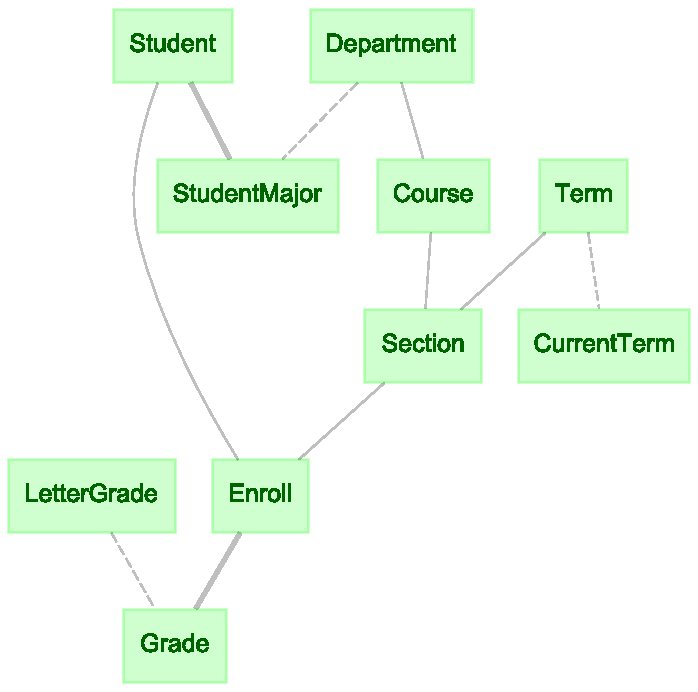
\includegraphics[width=\columnwidth]{uni_erd.pdf}
\caption{The schema diagram of the university database.}
\label{fig:erd}
\end{figure}


\subsubsection{Primary key}

\subsection{Dependencies}
\subsubsection{Effects of dependencies}\label{sec:effects}
Adding the dependency \lstinline$-> Ref$ to the definition of the new table \lstinline$Dependent$ has the following effects on the table definition: 
\begin{itemize}
\item The primary key attributes of $Ref$ are added to the definition of \lstinline$Depedent$ skipping those that are already present in the definition.
\item The referential constraint is created prohibiting tuples in \lstinline$Dependent$ without \emph{matching} entries in \lstinline$Ref$.
\item An index is created in \lstinline$Dependent$ to accelerate searches in \lstinline$Dependent$ given primary key values of \lstinline$Ref$.
\end{itemize}

The referential constraint works by (a) prohibiting inserts into \lstinline$Dependent$ of tuples that are missing the matching tuple in \lstinline$Ref$ and (b) propagating deletes from $Ref$ to $Dependent$ of all matching tuples.

\subsubsection{Primary and secondary dependencies}
\subsubsection{Acyclicity}

\subsection{Schema diagrams}\label{sec:diag}

\section{Data manipulation}\label{sec:manip}
\subsection{Insert}
\subsection{Delete}
\subsection{Cautious update}

\section{Query Expressions}\label{sec:query}
\subsection{Relational operators and expressions}
\begin{table*}[ht]
\begin{tabu}{|X|}
\hline
\hline
\end{tabu}
\caption{DataJoint query operators.}
\label{tab:operators}
\end{table*}

\subsection{Operational entity integrity}
\subsection{Join compatibility}
\subsection{Restriction}
\subsubsection{Restriction by attribute conditions}
\begin{lstlisting}[language=Python, caption={Restrictions by attribute conditions.}, label={lst:res1}]
# Students from Texas
Student & home_state == "TX"
# Students not from Texas
Student & home_state <> "TX"
Student \ home_state == "TX"
# Male students from outside Texas
Student & sex == "M" \ home_state == "TX"
\end{lstlisting}

\begin{lstlisting}[language=Python, caption={Assignment and use of relational variables.}, label={lst:res2}]
Millenial = Student & 
   date_of_birth >= "1980-01-01" & 
   date_of_birth < "2001-01-01"
MillenialMale = Millenial & sex == "M"
\end{lstlisting}

\subsubsection{Restriction by a mapping}

\subsubsection{Restriction by a collection}
\begin{lstlisting}[language=Python, caption={Restrictions by a collection of conditions.}, label={lst:res4}]
# Students from Texas, Oklahoma, or New Mexico
Student & [
   home_state == "OK", 
   home_state == "NM", 
   home_state == "TX"] 
\end{lstlisting}


\subsubsection{Restriction by a relation}
\begin{lstlisting}[language=Python, caption={Restrictions by another entity.}, label={lst:res5}]
# Students who have taken classes
Student & Enroll
# Students who have not taken classes
Student \ Enroll
# Students who have not selected a major
Student \ StudentMajor
\end{lstlisting}

\begin{lstlisting}[language=Python, caption={Composite restrictions.}, label={lst:res6}]
# Students who have taken Biology classes but no MATH courses
Student & 
  (Enroll & dept == "BIOL") \ 
  (Enroll & dept == "MATH")

# Students who are not taking courses in the current term
Student \ (Enroll & CurrentTerm)

# Students who have taken classes and have chosen a major
Student & Enroll & StudentMajor 

#Students who have taken classes or have chosen a major
Student & [Enroll, StudentMajor]
\end{lstlisting}

\begin{lstlisting}[language=Python, caption={Avoiding unintended restrictions.}, label={lst:res7}]
# Enrollment in courses from the same department as the students' major
Enroll & StudentMajor

# Enrollment not matching major 
Enroll \ StudentMajor 
\end{lstlisting}

\subsection{Join}
\begin{lstlisting}[language=Python, caption={Combining entities.}, label={lst:join1}]
# Grade point values
Grade * LetterGrade

# Graded enrollments with complete course and student information
Student * Enroll * Course * Section * Grade * LetterGrade
\end{lstlisting}

\begin{lstlisting}[language=Python, caption={Join in expressions.}, label={lst:join2}]
# Students with ungraded courses in current term
Student & (Enroll * CurrentTerm \ Grade)

# Enrollments before students' date of birth
Student * Enroll & (term_year <= date_of_birth)
\end{lstlisting}

\subsection{Projection}
\begin{lstlisting}[language=Python, caption={Selecting  attributes.}, label={lst:select}]
# Student name
Student.proj(first_name, last_name)
\end{lstlisting}

\begin{lstlisting}[language=Python, caption={Renaming attributes.}, label={lst:rename}]
# Enrollment with major information
Student.proj(first_name, last_name) * 
  Enroll * StudentMajor.proj(major: dept)

# Enrollement in courses by students that have selected a major
Enroll & StudentMajor.proj(major: dept)
\end{lstlisting}

\begin{lstlisting}[language=Python, caption={Projection in composite expressions.}, label={lst:proj}]
# Enrollment outside chosen major
Enroll * StudentMajor.proj(major: dept) & major <> dept
\end{lstlisting}

\begin{lstlisting}[language=Python, caption={Extension: calculated attributes.}, label={lst:extend}]
# Total grade points
(Course * Grade * LetterGrade).proj(
    total: points * credits)
\end{lstlisting}

\begin{lstlisting}[language=Python, caption={}]
# Total grade points in current term
(Course * Grade * LetterGrade).proj(
    total: points * credits) & CurrentTerm
\end{lstlisting}

\subsection{Union}

\subsection{Aggregation}
\begin{lstlisting}[language=Python, caption={Calculate summary statistics.}, label={lst:aggr1}]
# Students in each section
Section.aggr(Enroll, n: count(*))
\end{lstlisting}

\begin{lstlisting}[language=Python, caption={Aggregation in expressions.}, label={lst:aggr2}]
# Average grade in each course
Course.aggr(Grade*LetterGrade, avg_grade: avg(points))

# number of students enrolled per section
enrolled = Section.aggr(Enroll, n: count(*))

# number of students graded per section
graded = Section.aggr(Grade, m: count(*))

# fraction of enrolled students with grades
fraction = (enrolled * graded).proj(
    frac: m/n)

# Student GPA
graded = Course * Grade * LetterGrade
GPA = Student.aggr(graded,
    gpa: sum(points * credits)/
         sum(credits))

# Average GPA for each major
Department.aggr(StudentMajor * GPA, 
    avg_gpa: avg(gpa))
\end{lstlisting}

\begin{lstlisting}[language=Python, caption={Reuse of variables}, label={lst:aggr3}]
# GPA in current term
Student.aggr(graded & CurrentTerm, 
    gpa: sum(points * credits) / sum(credits))
\end{lstlisting}

Aggregation functions cannot be used in restrictions. 
\subsection{Relation U}
\begin{lstlisting}[language=Python, morekeywords={avg, U}, caption={Creating a new entity.}, label={lst:u1}]
# All home states
U(home_state) & Student

# Unique last names
U(last_name) & Student 
\end{lstlisting}

\begin{lstlisting}[language=Python, morekeywords={avg, U}, caption={Aggregation by a new entity.}, label={lst:u2}]
# Number of students from each state by sex
U(home_state, sex).aggr(Student, 
    n: count(*))

GPA = Student.aggr(sex,
    Course * Grade * LetterGrade,
    gpa: sum(points * credits) /
         sum(credits))

GpaBySex = U(sex).aggr(GPA, 
    avg_gpa: avg(gpa))
\end{lstlisting}

\begin{lstlisting}[language=Python, morekeywords={avg, U}, caption={Aggregation and restriction.}, label={lst:u3}]
# Gender neutral-names
SexRatio = U(first_name).aggr(Student, 
    fraction_male: avg(sex == "M")) 

GenderNeutral = SexRatio & 
    fraction_male > 0 & fraction_male < 1
\end{lstlisting}

\begin{lstlisting}[language=Python, morekeywords={avg, U}, caption={Elevation of a secondary attribute.}, label={lst:u4} ]
# Students with the same birthdays
s = Student.proj(date_of_birth, 
    other: student_id) * 
    U(date_of_birth)

SameBirthday = Student * s & 
    student_id < other
\end{lstlisting}

\section{Advanced schema definition}\label{sec:def2}
\subsection{Derived dependencies}
As described in Section \ref{sec:def1}, dependencies (foreign keys) are defined in table definitions using the arrow notation:
\begin{lstlisting}
-> Ref
\end{lstlisting}
In Section \ref{sec:def1} we only considered the case where \lstinline$Ref$ was a base relation. 
The DataJoint model generalizes dependencies to allow referencing derived relations (entity sets).

\subsection{Master-part relationship}
The primary motivation for the master-part relationship is to inform the application that the master and all its parts should always appear together or not at all.  
This usually means using transactions.  
A transaction starts then the master is inserted, then all the parts, and only then the transaction is committed.  
This way all other users only see the master entry when all its parts have been entered.
A part may be in 1-to-1 relationship with its master without any new primary attributes.

\subsection{Dependency properties}

\section{Discussion}
The relational model for databases has been around for nearly fifty years and its use has been standardized by the wide adoption of SQL.
However, some lack of conceptual clarity of SQL and the relational data model make them unwieldy for conceptual design and complex queries.
As a result, the field has converged on the understanding that database design consists of two distinct components: \emph{conceptual modeling} and \emph{logical modeling} leading to physical implementation. 
Although the Entity Relationship Model was proposed as a model suitable for both conceptual modeling and definition of database schemas, it never replaced the refined data definition languages and evolved into a tool limited to conceptual modeling.  
Furthermore, the ERM's conceptual clarifications chiefly pertain to schema definition and do not provide a data query language with the same level conceptual clarification for derived results as for stored data.

The relational data model and its query languages relational algebra and relational calculus are not concerned with observing. 
SQL is implemented to support the general unrefined relational data model while also deviating from it in significant ways. 

\section{Acknowledgements}
We conceived DataJoint in Andreas S.\ Tolias' lab in the Neuroscience Department at Baylor College of Medicine in the fall of 2009. 
Initially implemented as a thin MySQL API in MATLAB, it defined the major principles of the DataJoint model summarized here. 
Many students and postdocs in the lab as well as collaborators and early adopters have contributed to the project.
In particular, Alexander S.\ Ecker, Philipp Berens, Andreas Hoenselaar, and R.\ James Cotton contributed to the formulation of the overall requirements for the data model and critical reviews of DataJoint development.
Edgar Y.\ Walker and Fabian Sinz have been principal contributors to the DataJoint Python library. 
Jacob Reimer and Emmanouil Froudarakis became early adopters within Andreas Tolias' Lab and propelled development.
Outside the Tolias lab, the first labs to adopt DataJoint (approx.\ 2010) were the labs of Athanassios G.\ Siapas at CalTech, Laura Busse and Steffen Katzner at the University of T\"ubingen.
In 2017, DARPA awarded a small-business innovation research grant to Vathes LLC (Contract D17PC00162) to further develop and publicize the DataJoint framework. 

%\appendix
%\section{Entity normalization vs.\ Normal Forms}.

%\section{Differences from SQL}
%Faithful adherence to the relational data model. 
%Native entity integrity.

%\subsection{SQL Translations}


\bibliography{DataJoint}

\end{document}
